% ==================================================================================================================== %
% dune-fem-functionals.tex
% by: Felix Albrecht (felix.albrecht@uni-muenster.de)
%     Patrick Henning (patrick.henning@uni-muenster.de)
%     Stefan Girke (s_girk01@uni-muenster.de)
% ==================================================================================================================== %
\documentclass[a4paper,11pt]{article}

% required packages and definitions
\usepackage[utf8]{inputenc}
% \usepackage[body={148mm,240mm,nohead}]{geometry}

\usepackage{multicol}
\usepackage{xspace}
\usepackage{relsize}

\usepackage[usenames,dvipsnames]{pstricks}
\usepackage{epsfig}


\usepackage{amsmath}
\usepackage{amsfonts}
\usepackage{amsthm}
\numberwithin{equation}{section}
\newtheorem{definition}{Definition}[section]
\newtheorem{class}[definition]{Class}
\newtheorem{remark}[definition]{Remark}
\newtheorem{example}[definition]{Example}
\newtheorem{lemma}[definition]{Lemma}
\newtheorem{problem}[definition]{Problem}
\newcommand{\theoremNewline}{\hspace{1mm}\\}
\newcommand{\theoremEndLine}{\hspace{1mm}}
\newcommand{\theoremItemizeNewline}{\hspace{1mm}\vspace{-3mm}}

\usepackage{hyperref}
\usepackage{url}

\usepackage{longtable}
\usepackage{listings}
\lstset{language=C++,
basicstyle=\ttfamily\color{black}\footnotesize,
keywordstyle=\underbar,
identifierstyle=,
commentstyle=\color{blue},
stringstyle=\itshape\color{green},
numbers=left,
numberstyle=\tiny}
\newcommand{\Code}[1]{\texttt{#1}}
\newcommand{\code}[1]{\lstinline!#1!}
\newcommand{\CodeT}[1]{\textnormal{\texttt{#1}}}
\newcommand{\codeT}[1]{\textnormal{\lstinline!#1!}}

\usepackage{tikz}
\usepgflibrary{arrows}

\newcommand{\dune}{\textsc{Dune}\xspace}
\newcommand{\dunecommon}{\textsc{Dune-Common}\xspace}
\newcommand{\dunegrid}{\textsc{Dune-Grid}\xspace}
\newcommand{\duneistl}{\textsc{Dune-Istl}\xspace}
\newcommand{\dunelocalfunctions}{\textsc{Dune-Localfunctions}\xspace}

\newcommand{\dunefem}{\textsc{Dune-Fem}\xspace}
\newcommand{\dunefemfunctionals}{\textsc{Dune-Fem-Functionals}\xspace}
\newcommand{\dunepdelab}{\textsc{Dune-PDELab}\xspace}
\newcommand{\dumux}{\textsc{DuMu}$^\textrm{x}$\xspace}

\newcommand{\alugrid}{\textsc{ALUGrid}\xspace}
\newcommand{\alberta}{\textsc{ALBERTA}\xspace}

\newcommand{\albertagrid}{{\tt AlbertaGrid}\xspace}
\newcommand{\alusimplexgrid}{{\tt ALUSimplexGrid}\xspace}
\newcommand{\alucubegrid}{{\tt ALUCubeGrid}\xspace}
\newcommand{\aluconformgrid}{{\tt ALUConformGrid}\xspace}
\newcommand{\uggrid}{{\tt UGGrid}\xspace}
\newcommand{\onedgrid}{{\tt OneDGrid}\xspace}
\newcommand{\sgrid}{{\tt SGrid}\xspace}
\newcommand{\yaspgrid}{{\tt YaspGrid}\xspace}

\newcommand{\hnS}{\hspace{-1.25pt}}
\newcommand{\divergence}{\nabla\hnS\hnS\hnS\cdot}
\newcommand{\gradient}{\nabla\hnS\hnS}
\newcommand{\boundary}{\partial \hnS}
\newcommand{\dx}{\;d\hnS x}
\newcommand{\komma}{\text{,}}
\newcommand{\punkt}{\text{.}}
\newcommand{\K}{\mathbb{K}}
\newcommand{\N}{\mathbb{N}}
\newcommand{\R}{\mathbb{R}}
\newcommand{\Tau}{\mathcal{T}}

\title{Draft on \dunefemfunctionals}
\author{Felix Albrecht (\Code{felix.albrecht@uni-muenster.de}),\\
  Patrick Henning (\Code{patrick.henning@uni-muenster.de}) and\\
	Stefan Girke (\Code{s\_girk01@uni-muenster.de}).
}
\date{\today}

\begin{document}

  \maketitle

  \begin{abstract}
    This document is a draft about a new concept of \dunefem based on functionals. \dunefem is part of the
    Distributed and Unified Numerics Environment (\dune) and is available from
    \url{http://dune.mathematik.uni-freiburg.de/}.
  \end{abstract}

  \hrule

  \begin{small}
    \tableofcontents
  \end{small}

  \vspace{5mm}
  \hrule

  \section{Introduction}
    \label{section::introduction}

    The overall goal of \dunefem and \dunefemfunctionals is the efficient numerical solution of PDE's. We will present
    some examples in this section, that may serve as a design motivation.

    \subsection{finite element solution of elliptic boundary value problems}

    Assuming standard notation, the following elliptic PDE is one of the simplest sample problem we would like to solve
    with \dunefemfunctionals.

    \begin{example}[elliptic boundary value problem]\theoremNewline
      \label{example::introduction::elliptic_pde}
      Let ${\Omega \subset \R}$ be a bounded connected lipshitz-domain and let ${a\komma f : \Omega \rightarrow \R}$ and
      ${g : \boundary\Omega \rightarrow \R}$ be given functions. Find ${u: \Omega \rightarrow \R}$, such that
      \begin{align}
        \label{equation::introduction::elliptic_pde}
        - \divergence
          \big(
            a \gradient u
          \big)
          &= f &&\text{in } \Omega \komma
        \\
        u &= g &&\text{on } \boundary\Omega \punkt
        \notag
      \end{align}
    \end{example}\theoremEndLine

    \begin{definition}[weak formulation]\theoremNewline
      \label{definition::introduction::weak_formulation}
      Let $H^1$ and $H^1_0$ be given as usual and let the affine subspace $H^1_g$ be
      defined as
      \begin{align}
        H^1_g :=
          \big\{
            v \in H^1
          \big|
            v = v_0 + \hat{g} \text{ for a } v_0 \in H^1_0
          \big\}\komma
        \notag
      \end{align}
      where ${\hat{g} \in H^{1}}$ is a ${H^{1}}$ representation of $g$.
      The weak formulation of problem \eqref{equation::introduction::elliptic_pde} then reads as follows. Find
      ${u \in H^1_g}$, such that
      \begin{align}
        \label{equation::introduction::weak_formulation}
        \int\limits_{\Omega}
          a \gradient u \gradient v
        \dx
        =
        \int\limits_{\Omega}
          f v
        \dx
        &&\text{for all } v \in H^1_0 \punkt
      \end{align}
    \end{definition}\theoremEndLine

    The weak formulation \eqref{equation::introduction::weak_formulation} gives rise to the introduction of
    functionals and operators. A rigorous mathematical definition of these can be found in the next section.
    The following is only intended to give the basic idea.

    \begin{definition}[operator and functional]\theoremNewline
      \label{definition::introduction::operators_functionals}
      The function $f$ from he original problem \ref{equation::introduction::elliptic_pde} induces a functional
      \begin{align}
        F: H^1 &\rightarrow \R
          \notag\\
        v &\mapsto F[v] :=
          \int\limits_{\Omega}
            f v
          \dx\punkt
          \notag
        \intertext{Accordingly the function $a$ from the original problem \ref{equation::introduction::elliptic_pde}
          induces an operator}
        A: H^1 &\rightarrow H^{-1}
          \notag\\
        u &\mapsto A(u) \komma
          \notag
        \intertext{where $A(u)$ itself is a functional, defined by}
        A(u): H^1 &\rightarrow \R
          \notag\\
        v &\mapsto A(u)[v] :=
          \int\limits_{\Omega}
            a \gradient u \gradient v
          \dx\punkt
          \notag
      \end{align}
    \end{definition}\theoremEndLine

    With these definitions at hand the weak formulation \eqref{equation::introduction::weak_formulation} can be
    rewritten in the following way.

    \begin{remark}[variational problem]\theoremNewline
      \label{remark::introduction::variational_formulation_functionals_operators}
      Let $A$ and $F$ be as in definition \ref{definition::introduction::operators_functionals}. The weak formulation
      \eqref{equation::introduction::weak_formulation} can be rewritten as follows.
      Find ${u \in H^1_g}$, such that
      \begin{align}
        \label{equation::introduction::variational_formulation_functionals_operators}
        A(u)[v] = F[v] &&\text{for all } v\in H^1_0 \punkt
      \end{align}
    \end{remark}\theoremEndLine

    In order to solve the above problem, one can rewrite equation
    \eqref{equation::introduction::variational_formulation_functionals_operators} using the definition of the affine
    subspace.

    \begin{remark}[solution of the variational problem]\theoremNewline
      \label{remark::introduction::solution_of_the_variational_problem}
      With the notation from remark \ref{remark::introduction::variational_formulation_functionals_operators}, find
      ${u_{0} \in H^{1}_{0}}$, such that
      \begin{align}
        \label{equation::introduction::variational_formulation_in_h_1_0}
        A(u_{0})[v] = F[v] - A(\hat{g})[v] &&\text{for all } v\in H^1_0 \punkt
      \end{align}
      The solution ${u \in H^{1}_{g}}$ of \eqref{equation::introduction::variational_formulation_functionals_operators}
      is then given as
      \begin{align}
        \label{equation::introduction::solution}
        u := u_{0} + \hat{g}\punkt
      \end{align}
    \end{remark}\theoremEndLine

    \begin{definition}[finite element discretization]\theoremNewline
      \label{definition::introduction::finite_element_discretization}
      With the notation from above, let $\Tau_h$ be a conform admissable triangulation of the domain $\Omega$ with
      codim 0 elements ${T \in \Tau_h}$. The usual finite element lagrange spaces are then given by
      \begin{align}
        \label{equation::introduction::lagrange_space}
        S_{h}^{k} &:=
          \big\{
            v_{h} \in C^{0}(\Omega)
          \big|
            v_{h}|_{T} \in \mathbb{P}^{k}(T) \quad\forall T \in \Tau_{h}
          \big\}\komma\\
        {S_{h}^{k}}_{0} &:=
          \big\{
            v_{h} \in S_{h}^{k}
          \big|
            v_{h} = 0 \text{ on } \boundary \Omega
          \big\}
        \intertext{and}
        {S_{h}^{k}}_{g} &:=
          \big\{
            v_{h} \in S_{h}^{k}
          \big|
            {v_{h}}_0 + g_{h} \text{ for a } {v_h}_0 \in {S_h^k}_0
          \big\}\komma
      \end{align}
      where ${g_{h} \in S_{h}^{k}}$ is the projection of $\hat{g}$ onto ${S_{h}^{k}}$.
    \end{definition}\theoremEndLine

    With these discrete function spaces at hand, we can define the finite element solution to problem
    \eqref{equation::introduction::elliptic_pde}.

    \begin{definition}[finite element solution]\theoremNewline
      \label{definition::introduction::finite_element_solution}
      With the notation from above, find ${{u_{h}}_{0} \in {S_{h}^{1}}_0}$, such that
      \begin{align}
        \label{equation::introduction::finite_element_solution_0}
          A({u_{h}}_{0})[v_{h}] = F[v_{h}] - A(g_{h})[v_{h}] &&\text{for all } v_{h} \in {S_{h}^{1}}_0\punkt
      \end{align}
      The finite element solution ${u_h \in {S_h^1}_h}$ of \eqref{equation::introduction::elliptic_pde} is then given as
      \begin{align}
        \label{equation::introduction::finite_element_solution}
          u_{h} := {u_{h}}_{0} + g_{h}\punkt
      \end{align}
    \end{definition}\theoremEndLine

    The following algorithm gives rise to the corresponding constructs that we will nedd in \dunefemfunctionals.

    \begin{definition}[algorithm to solve the elliptic boundary value problem]\theoremNewline
      This algorithm computes the finite element solution of problem
      \eqref{equation::introduction::elliptic_pde}.
      \begin{itemize}
        \item[$(i)$] define the finite element space $S_{h}^{1}$
        \item[$(ii)$] define the test space ${S_{h}^{1}}_{0} \subset S_{h}^{1}$ as a linear subspace
        \item[$(iii)$] define the ansatz space ${S_{h}^{1}}_{g} \subset S_{h}^{1}$ as an affine subspace
        \item[$(iv)$] define the operator ${A: {S_{h}^{1}} \rightarrow {S_{h}^{1}}^{-1}}$
        \item[$(v)$] define the functional ${F \in {S_{h}^{1}}^{-1}}$
        \item[$(vi)$] assemble a matrix with entries
          \begin{align}
            \label{equation::introduction::matrix_entries}
            (A)_{i,j} := A( \varphi_{i} )[ \psi_j ]
          \end{align}
          for all basefunctions of the ansatz-space ${\varphi_i \in S_{hg}^1}$ and all basefunctions of the test-space
          ${\psi_j \in {S_h^1}_0}$
        \item[$(vii))$] assemble a vector with entries
          \begin{align}
            \label{equation::introduction::vector_entries}
            (F)_{j} := F[ \psi_j ]
          \end{align}
          for all basefunctions of the test-space ${\psi_j \in {S_h^1}_0}$
        \item[$(viii)$] solve the algebraic system
          \begin{align}
            \label{equation::introduction::algebraic_system}
            A x = F
          \end{align}
          for $x$
        \item[$(ix)$] compute the solution ${u \in S_{hg}^{1}}$ as
          \begin{align}
            \label{equation::introduction::algebraic_solution}
            u_h := u_{h0} + \hat{g}\komma
          \end{align}
          where ${u_{h0} \in S_{h0}^{1}}$ is the discrete function belonging to the dof vector $x$.
      \end{itemize}
    \end{definition}


  \section{Abstract concept}
    \label{section::abstract_concept}

    \subsection{Functionals}

      We start with an overview on the mathematical concept which is carried over to a corresponding programming
      concept. The following notations and definitions are required for the subsequent sections.

      \begin{definition}[Function and Functionspace]\theoremNewline
        \label{definition::abstract_concept::function_functionspace}
        Let ${n,d \in \N^{\geq 1}}$ be integers and ${\Omega \subseteq \mathbb{R}^n}$ a subset. A mapping
        ${v : \Omega \rightarrow \R^d}$ is called a \textnormal{function}, the set
        \begin{align}
          V :=
            \big\{
              v : \Omega \rightarrow \R^d
            \big\}
            \notag
        \end{align}
        is called a \textnormal{functionspace}. If $V$ is an $\R$--vector space, $V$ is called a \textnormal{linear functionspace}.
      \end{definition}\theoremEndLine

      \begin{definition}[Functional]\theoremNewline
        \label{definition::abstract_concept::functional}
        Let $V$ be a function space. A map
        \begin{align}
          F: V &\rightarrow \R\komma
            \notag\\
          v &\mapsto F[v]
        \end{align}
        is called a \textnormal{Functional}. If
        \begin{align}
          F[\alpha v_1 + \beta v_2] = \alpha F[v_1] + \beta F[v_2]
            \notag
        \end{align}
        holds for all ${\alpha,\beta \in \R}$ and all ${v_1,v_2\in V}$, $F$ is called a \textnormal{linear Functional}.
        The vector space
        \begin{align}
          V' := \big\{ F : V \rightarrow \R \big| F \text{ is a linear functional } \big\}
        \end{align}
        is called the dual space of $V$.
      \end{definition}\theoremEndLine

      \begin{lemma}[Localization property of discrete linear functionals]\theoremNewline
        \label{lemma::abstract_concept::localization_property_of_discrete_linear_functionals}
        Let $V_G$ be a discrete function space (\cite[Def. 18]{DKNO10}) and ${F \in V_G'}$ a discrete linear functional.
        Let further be
        \begin{align}
          u &= \sum\limits_{E \in G}
              {
                u_E
              }
          \intertext{the representation for a ${u \in V_G}$ in terms of its local functions ${u_E := u_{|E}}$ and}
          u_E &= \sum\limits_{i \in I_E}
              {
                u_i^E \varphi_i^E
              }
        \end{align}
        the representation of a local function in terms of its local DoFs $u_i^E$ and the local
        base functions $\varphi_i^E$ (\cite[Def. 20]{DKNO10}). Thus, $u_E$ can be written as
        \begin{align}
          u &= \sum\limits_{E \in G}
              {
                \sum\limits_{i \in I_E}
                {
                  u_{\mu_G(i)}^E \varphi_{\mu_G(i)}^E
                }
              }\komma
            \notag
        \end{align}
        where ${\mu_G}$ is local--to--global DoF mapping (\cite[Def. 18]{DKNO10}). Since $F$ is a discrete linear functional, it holds that
        \begin{align}
          F[u] &= \sum\limits_{E \in G}
              {
                \sum\limits_{i \in I_E}
                {
                  u_{\mu_G(i)}^E F \Big[ \varphi_{\mu_G(i)}^E \Big]
                }
              }\komma
          \intertext{which can also be written as}
          F[u] &= \sum\limits_{E \in G}
              {
                u^E \cdot F[B_E]^E
              }\komma
        \end{align}
        where $u^E := ( u_{\mu_G(i)}^E )_{i \in I_E}$ is the local DoF vector of $u_E$ (mapped to global) and
        ${F[B_E]^E}$ is defined as the vector
        \begin{align}
          F[B_E]^E := \Bigg( F \Big[ \varphi_{\mu_G(i)}^E \Big] \Bigg)_{i \in I_E}
        \end{align}
        for a local basefunction set $B_E$.
      \end{lemma}\theoremEndLine

      An important set of linear functionals is the set of those functionals that are associated with integration, e.g
      the functional $F$, induced by the function $f$, which arises as a right hand side in the introductory example
      (see definition \ref{definition::introduction::operators_functionals}). To formulate the abstract idea of an
      ``integral functional'', we first have to introduce a ``codim $c$ functional``, which is associated with integration
      over a set of codimension $c$.

      \begin{definition}[Codim $c$ functional]\theoremNewline
        Let $V_G$ be a discrete function space and ${F \in V_G'}$ a discrete linear functional. If ${F[v]}$ can be
        written as
        \begin{align}
          F[v] &= \int\limits_{\omega^c}
              {
                \tilde{f}[v](x) \dx
              }
            \notag
        \intertext{for a function ${v \in V_G}$, a subset ${\omega^c \subset \Omega}$ of codimension $c$ and a map}
          \tilde{f} :& V_G \rightarrow V_G \komma
            \notag
        \end{align}
        $F$ is called a \textnormal{codim $c$ functional}. The map $\tilde{f}$ is called a
        \textnormal{local operation provider}.
      \end{definition}\theoremEndLine

      Given suitable codim $c$ functionals for all codimensions of interest we can now define an integral functional
      as a combination of those codim $c$ functionals.

      \begin{definition}[Integral functional]\theoremNewline
        Let $V_G$ be a discrete function space, ${F^{c_1}\komma \dots \komma F^{c_C} \in V_G'}$ codim functionals for
        the codimensions ${c_1 \komma \dots \komma c_C \in \N^{\geq 0}}$ and ${F \in V_G'}$ a discrete linear
        functional. If $F[v]$ can be written as
        \begin{align}
          F[v] = \sum\limits_{c=c_1}^{c_C}
              {
                F^{c}[v]
              }
            \notag
        \end{align}
        for a function ${v \in V_G}$, $F$ is called an \textnormal{integral functional}.
      \end{definition}\theoremEndLine

      \begin{remark}[Localization property of integral and codim $c$ functionals]
        Since integral functionals and codim $c$ functionals are themselves discrete linear functionals we can localize
        the evaluation of these functionals as in lemma
        \ref{lemma::abstract_concept::localization_property_of_discrete_linear_functionals}.
      \end{remark}




    \subsection{Constraints and subspaces}

    \begin{definition}[Constraint]\theoremNewline
      \label{definition::abstract_concept::constraint}
      Let $V$ be a linear function space, $M \in \mathbb{N}_{>0}$ and $\{ F_1, ..., F_M \}$ a set of linear
      functionals on $V$. We define the corresponding vector of linear functionals $C$ by
      \begin{align}
        C: \{1,...,M\} \times V &\rightarrow \R \enspace \mbox{with} \enspace (i,v) \mapsto C[i][v] := F_i[v].
      \end{align}
      The condition:
        \begin{align}
        C[i][v] = 0 \enspace \forall 1 \le i \le M
        \end{align}
      is called a \textnormal{Constraint} for $v$.
    \end{definition}

    In particular each linear functional implies a constraint.

    \begin{definition}[Linear subspace]\theoremNewline
      \label{definition::abstract_concept::linear_subspace}
      Let $V$ be a linear function space and $C[\cdot][\cdot]=0$ a constraint on $V$. Then we call
      \begin{align}
        V_C := \{ v \in V| \hspace{4pt} C[i][v] = 0 \hspace{4pt}\forall i\in\{1,...,M\}\}
      \end{align}
      a \textnormal{linear subspace} of $V$ with respect to $C$.
    \end{definition}

    $V_C$ is a vector space itself, since the constraint functionals $C[i]$ are linear. Typically, $V_C$ becomes the
    space of test functions in our later problem.

    \begin{definition}[Affine subspace]\theoremNewline
      \label{definition::abstract_concept::affine_space}
      Let $V$ be a function space, $V_C$ a linear subspace and $g \in V$. Then we call
      \begin{align}
        V_{g} := \{ v+g| \hspace{4pt} v \in V_C \} \subset V
      \end{align}
      an \textnormal{affine subspace} with respect to $g$ and $V_C$.
    \end{definition}\theoremEndLine

    In general, $V_g$ is only a subspace of $V$ and not a linear subspace (in the sense, that $V_G$ is not a vector
    space itself in general ). It will be the space of solutions in our later problem.

    \subsection{Operators}

    \begin{definition}[Operator]\theoremNewline
      \label{definition::abstract_concept::operator}
      Let $V$ be a linear function space, ${V_C \subset V}$ a linear subspace, $V_C'$ its dual and ${V_g \subset V}$
      an affine subspace. Then we call
      \begin{align}
        G : V_g \rightarrow V^{\prime}_C
      \end{align}
      an \textnormal{operator} on $V_g$. If
      \begin{align}
        G(\alpha v + \beta w) = \alpha G(v) + \beta G(w)
          \notag
      \end{align}
      holds for all ${\alpha\komma \beta \in \R}$ and for all ${v\komma w \in V_g}$ the operator $G$ is called
      \textnormal{linear}.
    \end{definition}

    In the subsequent sections, we are dealing with the following problem.

    \begin{problem}[Sample problem]\theoremNewline
      \label{problem::abstract_concept::sample_problem}
      Let $V$ be a linear space, ${V_C \subset V}$ a linear subspace, ${F \in V_C'}$ a functional and
      ${V_g \subset V}$ an affine subspace. Find ${u \in V_g}$, such that
      \begin{align*}
        G(u)[v] = F[v] &&\text{for all } v \in V_C.
      \end{align*}
    \end{problem}

    In general, the functional $F$ on the right hand side of our problem is linear. The (differential) operator $G$
    can be either linear or nonlinear.

  \section{Examples}
    \label{section::examples}

    \subsection{Elliptic PDE}

      Let $\Omega \subset \mathbb{R}^d$ denote a polygonal bounded domain, $\mathcal{T}_H = \{ T_1, ..., T_N \}$ a
      corresponding regular triangulation, $\mathcal{N}_H = \{ x_1, ...., x_{\tilde{N}}\}$ the set of nodes and
      $\{ \Phi_1, ...., \Phi_{\tilde{N}}\}$ the associated Lagrange basis of order $1$. The (discrete) linear space of
      solutions is given by
      \begin{align*}
        V :=
          \Big\{
            v_H \in C^0(\Omega)
          \Big|
            (v_H)_{|T}\in \mathbb{P}^1(T) \quad\forall T \in \mathcal{T}_H
          \Big\}
      \end{align*}
      and the linear subspace of testfunctions by $V_0 := V \cap H^1_0(\Omega)$. Now, let us consider the
      following discrete problem.

      \begin{problem}\theoremNewline
      For $g \in V$ find $u \in V$ with $u=g$ on $\partial \Omega$ and
      \begin{align*}
      \int\limits_{\Omega} \nabla u \cdot \nabla v \dx = \int\limits_{\Omega} f v \dx &&\text{for all }v \in V_0.
      \end{align*}
      (Note: $V_0$ can not be replaced by $V$).
      \end{problem}

      Putting this into the general framework above, we define the (linear) functional
      ${F: V_0 \rightarrow \R}$ by
      \begin{align*}
        F[v] := \int\limits_{\Omega} f v &&\text{for } v \in V_0.
      \end{align*}
      $V_0$ is a constraint subspace with the constraint $C[i][v] := v(x_i^b) = 0$ for any boundary node
      $x_i^b$ (i.e. $\mathcal{N}_H \cap \partial \Omega = \{ x_1^b, ...., x_{\bar{N}}^b\}$). We can therefore identify
      \begin{align*}
        V_0 = \{ v \in V| \hspace{3pt} C[i][v] = 0 \enspace \forall 1\le i\le \bar{N} \} =: V_C.
      \end{align*}
      The affine subspace $V_{g_H}$is given by
      \begin{align*}
        V_{g_H} :=
          \Big\{
            v + g_H
          \Big|
            v \in V \enspace \mbox{and} \enspace g_H := \sum_{i=1}^{\tilde{N}} g(x_i) \Phi_i
          \Big\}
      \end{align*}
      and the (differential) operator $G : V_{g_H} \rightarrow V_C^{\prime}$ by
      \begin{align*}
      G(u)[v] := \int_{\Omega} \nabla u \cdot \nabla v \dx.
      \end{align*}
      With these notations the original problem reads:
      \begin{align*}
      \text{Find} \enspace u \in V_{g_H} \enspace \mbox{with} \enspace G(u) = F \enspace \mbox{on} \enspace V_C.
      \end{align*}

  \section{Realization in \dunefemfunctionals}
    \label{realization_in_dune_fem_dunctionals}

    In this section we describe the general programming concept. For a detailed description of these classes, see
    section ? and the doxygen documentation. These classes are realized in a namespace \Code{Functionals} in order to
    avoid conflicts with other existing \dunefem-classes. We do not distinguish between interfaces and realizations
    here, this is only intended as a conceptual overview.

    \subsection{Functionals}

      The following diagram is intended to be a conceptual overview only. It is not intended to display a class
      hierarchy.

      \begin{remark}[Conceptual class tree]\theoremNewline
        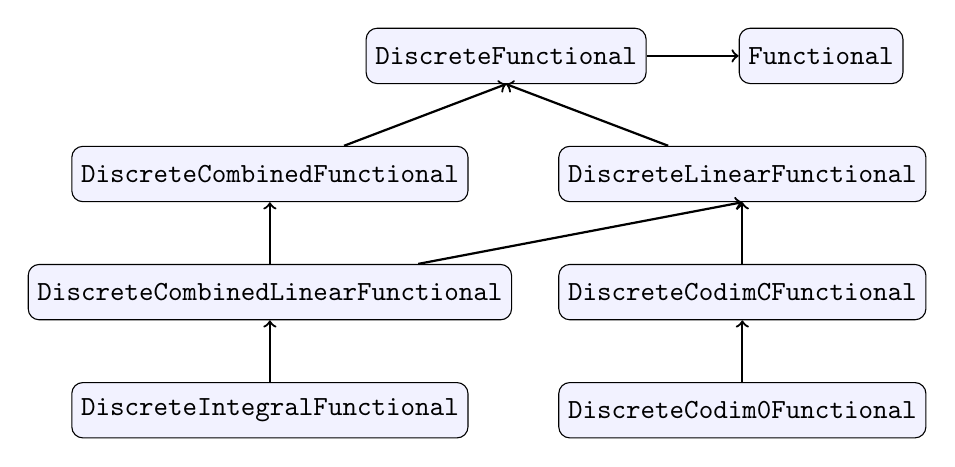
\begin{tikzpicture}
          \tikzstyle{boxs} = [draw, %text width=4em,
            fill=blue!5, minimum height=2em, rounded corners]
          \tikzstyle{boxsG} = [draw,  %text width=4em,
            fill=green!5, minimum height=2em, rounded corners ]
          \tikzstyle{line} = [draw,->,thick]
          \tikzstyle{lineR} = [draw,<-,thick]

          \tikzset{node distance = 40mm}
          \node(Functional)[boxs]{\CodeT{Functional}};

          \node(DiscreteFunctional)[boxs,left of = Functional]{\CodeT{DiscreteFunctional}} edge[line] (Functional.west);

          \tikzset{node distance = 15mm}
          \node(dummy1)[below of = DiscreteFunctional]{};
          \tikzset{node distance = 30mm}
          \node(DiscreteCombinedFunctional)[boxs,left of = dummy1]{\CodeT{DiscreteCombinedFunctional}} edge[line] (DiscreteFunctional.south);
          \node(DiscreteLinearFunctional)[boxs,right of = dummy1]{\CodeT{DiscreteLinearFunctional}} edge[line] (DiscreteFunctional.south);

          \tikzset{node distance = 15mm}
          \node(DiscreteCombinedLinearFunctional)[boxs,below of = DiscreteCombinedFunctional]{\CodeT{DiscreteCombinedLinearFunctional}} edge[line] (DiscreteCombinedFunctional.south) edge[line] (DiscreteLinearFunctional.south);

          \node(DiscreteCodimCFunctional)[boxs,below of = DiscreteLinearFunctional]{\CodeT{DiscreteCodimCFunctional}} edge[line] (DiscreteLinearFunctional.south);

          \node(DiscreteCodim0Functional)[boxs,below of = DiscreteCodimCFunctional]{\CodeT{DiscreteCodim0Functional}} edge[line] (DiscreteCodimCFunctional.south);

          \node(DiscreteIntegralFunctional)[boxs,below of = DiscreteCombinedLinearFunctional]{\CodeT{DiscreteIntegralFunctional}} edge[line] (DiscreteCombinedLinearFunctional.south);
        \end{tikzpicture}
      \end{remark}\theoremEndLine

      The class \Code{Functional} will not really be used. It is only there to provide us with the possibility to have
      all the following classes in a non--discrete way in the future. The only thing this class does is to enforce the
      \Code{operator()} for all functionals. The only method, the function $v$ has to provide, is a method
      \Code{evaluate( xGlobal )}.

      \begin{class}[\CodeT{Functional}]\theoremNewline
        This class represents a functional $F$ (see definition \ref{definition::abstract_concept::functional}). It
        provides the base class for discrete and what--ever--else--there--will--be functionals.\\\\
        \begin{tabular}{l}
          \textbf{Class definition:}\\
          \hline
          \hline
          \codeT{class Functional< FunctionSpaceType >}
        \end{tabular}\\\\\\
        \noindent
        \begin{longtable}{l}
          \textbf{Methods:}\\
          \hline
          \hline
          \CodeT{RangeFieldType ret = operator(}\\
          \CodeT{ FunctionType function )}\\
          \begin{tabular}{l|l}
            description:
              & This method represents the functional, applied to a function.\\
            \hline
            in:
              & \begin{tabular}{ll}
                  \codeT{FunctionType function}
                  & $v$
                \end{tabular}\\
            \hline
            out:
              & \begin{tabular}{ll}
                  \codeT{RangeFieldType ret}
                  & ${F[v]}$
                \end{tabular}
          \end{tabular}
        \end{longtable}
      \end{class}\theoremEndLine

      The class \Code{DiscreteFunctional} is the actual base class for all functionals we use at the time being.

      \begin{class}[\CodeT{DiscreteFunctional}]\theoremNewline
        This class represents a functional $F$ (see definition \ref{definition::abstract_concept::functional}),
        which can be applied to a discrete function.\\\\
        \begin{tabular}{l}
          \textbf{Class definition:}\\
          \hline
          \hline
          \codeT{class DiscreteFunctional< DiscreteFunctionSpaceType >}
        \end{tabular}\\\\\\
        \noindent
        \begin{longtable}{l}
          \textbf{Methods:}\\
          \hline
          \hline
          \CodeT{RangeFieldType ret = operator(}\\
          \CodeT{ DiscreteFunctionType discreteFunction )}\\
          \begin{tabular}{l|l}
            description:
              & This method represents the functional, applied to a function.\\
            \hline
            in:
              & \begin{tabular}{ll}
                  \codeT{FunctionType function}
                  & $v$
                \end{tabular}\\
            \hline
            out:
              & \begin{tabular}{ll}
                  \codeT{RangeFieldType ret}
                  & ${F[v]}$
                \end{tabular}
          \end{tabular}
        \end{longtable}
      \end{class}\theoremEndLine

      The \Code{DiscreteCombinedFunctional} is more or less a pair of two \code{DiscreteFunctional}s. When its
      \Code{operator()} is called, it just calls each \Code{operator()} and adds the results.

      \begin{class}[\CodeT{DiscreteCombinedFunctional}]\theoremNewline
        Given two functionals ${F \komma G \in V'}$, this class represents the functional
        \begin{align}
          F+G: V &\rightarrow  \R
            \notag\\
          v &\mapsto F[v] + G[v]\punkt
            \notag
        \end{align}
        This class is derived from \codeT{DiscreteFunctional}.\\\\
        \begin{tabular}{l}
          \textbf{Class definition:}\\
          \hline
          \hline
          \CodeT{class DiscreteCombinedFunctional< }\\
          \CodeT{ FirstFunctionalType,}\\
          \CodeT{ SecondFunctionalType >}\\
          \CodeT{ : Functional}
        \end{tabular}\\\\\\
        \noindent
        \begin{longtable}{l}
          \textbf{Methods:}\\
          \hline
          \hline
          \CodeT{RangeFieldType ret = operator(}\\
          \CodeT{ DiscreteFunctionType discreteFunction )}\\
          \begin{tabular}{l|l}
            description:
              & This method redefines \codeT{DiscreteFunctional::operator()}.\\
            \hline
            in:
              & \begin{tabular}{ll}
                  \codeT{DiscreteFunctionType discreteFunction}
                  & $v$
                \end{tabular}\\
            \hline
            out:
              & \begin{tabular}{ll}
                  \codeT{RangeFieldType ret}
                  & ${F[v] + G[v]}$
                \end{tabular}
          \end{tabular}
        \end{longtable}
      \end{class}\theoremEndLine

      The \Code{DiscreteLinearFunctional} is the base class for a wide range of interesting functionals -- linear
      functionals. As stated in lemma
      \ref{lemma::abstract_concept::localization_property_of_discrete_linear_functionals},
      the most important property of linear functionals is, that its application to a discrete function can be split up
      and carried out by some kind of local application of the functionals to a local function.

      \begin{class}[\CodeT{DiscreteLinearFunctional}]\theoremNewline
        This class represents a linear functional $F$ (see definition \ref{definition::abstract_concept::functional}).
        All linear functionals have to provide the method \CodeT{applyLocal()} in addition to the method
        \CodeT{operator()}. This class is derived from \codeT{DiscreteFunctional}.\\\\
        \begin{tabular}{l}
          \textbf{Class definition:}\\
          \hline
          \hline
          \codeT{class DiscreteLinearFunctional< DiscreteFunctionSpaceType >}\\
          \codeT{: DiscreteFunctional}
        \end{tabular}\\\\\\
        \noindent
        \begin{longtable}{l}
          \textbf{Methods:}\\
          \hline
          \hline
          \CodeT{RangeFieldType ret = operator(}\\
          \CodeT{ DiscreteFunctionType discreteFunction )}\\
          \begin{tabular}{l|l}
            description:
              & This method redefines \codeT{DiscreteFunctional::operator()}.\\
              & It makes use of the localization property of linear\\
              & functionals (see lemma
                \ref{lemma::abstract_concept::localization_property_of_discrete_linear_functionals}). It is implemented
                as a grid\\
              & walk over all codim 0 entities which calls the method\\
              & \CodeT{applyLocal()} on each entity. Thus each linear functional\\
              & only has to implement the method \CodeT{applyLocal()}.\\
            \hline
            in:
              & \begin{tabular}{ll}
                  \codeT{DiscreteFunctionType discreteFunction}
                  & $v$
                \end{tabular}\\
            \hline
            out:
              & \begin{tabular}{ll}
                  \codeT{RangeFieldType ret}
                  & ${F[v]}$
                \end{tabular}
          \end{tabular}\\
          \hline
          \hline
          \CodeT{void applyLocal(}\\
          \CodeT{ LocalBasefunctionSetType localBasefunctionSet,}\\
          \CodeT{ LocalDoFVectorType returnVector )}\\
          \begin{tabular}{l|l}
            description:
              & Given the localization property of a linear functional (see\\
              & lemma \ref{lemma::abstract_concept::localization_property_of_discrete_linear_functionals}), this method
                implements the vector ${F[B_E]^E}$.\\
              & This is still only a rough idea of this methods signature.\\
              & It is highly possible that we will need to extend this method\\
              & to take additional arguments, such as the neighbors local\\
              & basefunction set etc...\\
            \hline
            in:
              & \begin{tabular}{ll}
                  \codeT{LocalBasefunctionSetType localBasefunctionSet}\\
                  $B_E$
                \end{tabular}\\
            \hline
            out:
              & \begin{tabular}{ll}
                  \codeT{LocalDoFVectorType returnVector}\\
                  ${F[B_E]^E := \Big( F \Big[ \varphi_{\mu_G(i)}^E \Big] \Big)_{i \in I_E}}$
                \end{tabular}
          \end{tabular}
        \end{longtable}
      \end{class}\theoremEndLine


\subsection{Required classes}

First of all we give an overview on the various classes that are required in our concept. In particular we comment on the functionality of each class.\\
\\
\noindent\CodeT{typedef Constraint < FunctionalType > ConstraintType;}
\begin{itemize}
	\item[$\circ$] various realizations of constraints $C$ are possible (boundary conditions, periodicity, zero-average, ...); they are derived from the general \CodeT{Constraint} class
	\item[$\circ$] mapping an element $v\in V$ on an element $v_C \in V_C$ is not unique, therefore 'applying a constraint' to a general function $v$ means that we project $v$ on $V_C$ with respect to certain scalar product; in the discrete setting these projections are typically straight forward
	\item[$\circ$] required methods:
	\item[$\cdot$] method: \CodeT{apply( numberOfConstraint, discreteFunction )} $\leftrightarrow$ find $v_C \in V_C$ which is 'close' to $v_H$ and which fulfills $C[i][v_C]=0$, $i$ is the index of the functional (in our functional vector), $v_H$ is a discrete function; typically we simply change the value of $v_H$ in a certain number of nodes
	\item[$\cdot$] method: \CodeT{applyLocal( numberOfConstraint, localBasefunctionSet, \\ localBasefunctionSet )} $\rightarrow$ again, an abstract method depending on the specific type of the constraint; it returns local contributions for a specific grid element; it is required for assembling the system matrix in our system of equations; details are given later
	\item[$\cdot$] method: \CodeT{applyLocal( localBasefunctionSet, localBasefunctionSet )} $\rightarrow$ use \CodeT{applyLocal( numberOfConstraint, localBasefunctionSet, \\ localBasefunctionSet )} for all \CodeT{numberOfConstraint}
	\item[$\circ$] other methods depending on the specific type of a constraint (e.g. DirichletConstraint)?
	\item[$\circ$] constraints are used to construct a 'constraint subspace' - for the user, nothing else has to be done with the constraints
\end{itemize}
\noindent\CodeT{typedef LinearSubspace < DiscreteFunctionSpace, ConstraintType >}
\CodeT{LinearSubspaceType;}
\begin{itemize}
	\item[$\circ$] derived from \CodeT{DiscreteFunctionSpace}
	\item[$\circ$] all the information about the constraint is in our subspace
	\item[$\circ$] we can extract the constraint that it was constructed from
	\item[$\circ$] formally the subspace is of the same size as \CodeT{DiscreteFunctionSpace}
	\item[$\circ$] in particular an object of \CodeT{LinearSubspace} becomes the space of test functions in our later problem
\end{itemize}
\noindent\CodeT{typedef AffineSubspace < LinearSubspace, DiscreteFunctionType >} \CodeT{AffineSubspaceType;}
\begin{itemize}
	\item[$\circ$] the space of the solution
	\item[$\circ$] initialized with a fixed discrete function $v_H$: 'AffineSubspace = $v_H$ + LinearSubspace'
	\item[$\circ$] \CodeT{AffineSubspace}-class derived from \CodeT{DiscreteFunctionSpace}
\end{itemize}
\noindent\CodeT{typedef Operator< LinearSubspaceType, AffineSubspaceType,}
\CodeT{MatrixObjectTraits > DifferentialOperatorType;}
\begin{itemize}
	\item[$\circ$] can be derived from the dune-fem Operator-class, later it should be implemented independently
	\item[$\circ$] Operator : AffineSubspace $\rightarrow$ (LinearSubspace$)^{\prime}$
	\item[$\circ$] if required: automatically assembles the correct system matrix (which is a quadratic sparse row matrix) with respect to the subspaces (i.e. with respect to the constraints)
	\item[$\circ$] simplified we can say: the {\it linear subspace} tells us which lines we must substitute in our later system of equations and the {\it affine subspace} tells us by what we must substitute these lines.
	\item[$\circ$] usage of a \CodeT{DifferentialOperatorType}-object identical to the old usage of an \CodeT{Operator}-object
	\item[$\circ$] {\it Algebraic representation:} get system matrix with \CodeT{operator.systemMatrix();} or \CodeT{operator.algebraic();}
%----------------------
%added by Stefan
%----------------------
	\item[$\circ$] incorporates something like:\\
	\CodeT{SystemMatrix(); constraints.apply( systemMatrix() );}, \CodeT{algebraic(); constraints.apply( algebraic() );} respectively
\end{itemize}

%-------------------------
%new version (Stefan)
%-------------------------
\noindent\CodeT{typedef FunctionalAssembler< FunctionalType, AffineSubspace >}\\
\CodeT{FunctionalAssemblerType;}
\begin{itemize}
	\item[$\circ$] assembles the right hand side in our system of equations
  \item[$\circ$] {\it Algebraic representation:} get assembled functional with \CodeT{functional.algebraic()}
  \item[$\circ$] incorporates something like:\\
\CodeT{algebraicl(); constraints.apply( functional );}
\end{itemize}

Both classes (\CodeT{DifferentialOperator} and \CodeT{FunctionalAssembler}) might be incorporated in a general \CodeT{FunctionalSolverInterface}, so that the user does not need to care about the system assemblers.

%--------------
%old version
%--------------
%Algebraic classes (assembling of system matrix and right hand side):\\
%\\
%To assemble the right hand side in our system of equations:\\
%\CodeT{typedef FunctionalAssembler < FunctionalType, AffineSubspace >

%FunctionalAssemblerType;}\\
%\\
%To assemble the correct system matrix (with respect to the subspaces):\\
%\CodeT{typedef OperatorAssembler < DiffOperatorType > OperatorAssemblerType;}
%\begin{itemize}
%\item incorporates something like:\\
%\CodeT{assembleSystemMatrix(); constraints.apply( systemMatrix() );}\\
%\end{itemize}
%Both classes might be incorporated in a general \CodeT{FunctionalSolverInterface}, so that the user does not need to care about the system assemblers.


%----------------------
%added by Stefan
%----------------------
\subsubsection{Suggestion for an alternative ''Assembler`` design}

Maybe we should think about the operator and ''assembled functional'' design again. Here is another abstract approach:\\

\begin{remark}[Conceptual class tree]\theoremNewline
		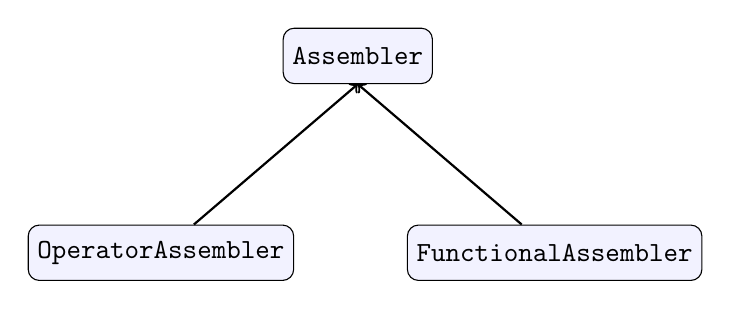
\begin{tikzpicture}
			\tikzstyle{boxs} = [draw, %text width=4em,
				fill=blue!5, minimum height=2em, rounded corners]
			\tikzstyle{boxsG} = [draw,  %text width=4em,
				fill=green!5, minimum height=2em, rounded corners ]
			\tikzstyle{line} = [draw,->,thick]
			\tikzstyle{lineR} = [draw,<-,thick]

			\node(Assembler)[boxs]{\CodeT{Assembler}};
			\tikzset{node distance = 25mm}
			\node(dummy1)[below of = Assembler]{};
			\node(OperatorAssembler)[boxs,left of = dummy1]{\CodeT{OperatorAssembler}} edge[line] (Assembler.south);
			\node(FunctionalAssembler)[boxs,right of = dummy1]{\CodeT{FunctionalAssembler}} edge[line] (Assembler.south);
			\tikzset{node distance = 15mm}

		\end{tikzpicture}
	\end{remark}\theoremEndLine

\noindent\CodeT{typedef Assembler < AssemblerTraits > AssemblerType;}
\begin{itemize}
	\item[$\circ$] Assembler interface class.
	\item[$\circ$] Each class derived from this interface defines a type \CodeT{AlgebraicRepresentationType}, which defines how the algebraic representation is stored - for example a vector or matrix.
	\item[$\circ$] A method \CodeT{algebraic()} with return type \CodeT{AlgebraicRepresentationType} is introduced here.
\end{itemize}

\noindent\CodeT{typedef OperatorAssembler< LinearSubspaceType, AffineSubspaceType>}\\
\CodeT{OperatorAssemblerType;}
\begin{itemize}
	\item[$\circ$] Derived from \CodeT{Assembler}.
	\item[$\circ$] \CodeT{typedef MatrixObject AlgebraicRepresentationType}.
	\item[$\circ$] The method \CodeT{algebraic()} represents the algebraic representation for the system matrix, i.e. the assembled system matrix.
\end{itemize}

\noindent\CodeT{typedef FunctionalAssembler < FunctionalType, AffineSubspace >}\\
\CodeT{FunctionalAssemblerType;}
\begin{itemize}
	\item[$\circ$] Derived from \CodeT{Assembler}.
	\item[$\circ$] \CodeT{typedef VectorObject AlgebraicRepresentationType}.
	\item[$\circ$] The method \CodeT{algebraic()} represents the algebraic representation, i.e. the assembled functional.
\end{itemize}

\noindent No we can define the \CodeT{Operator} and \CodeT{FunctionalAssembler} in a different way:

\noindent\CodeT{typedef Operator< FunctionalType, AffineSubspace,}
\CodeT{AssemblerType > DifferentialOperatorType;}\\
Note: We can also define \CodeT{typedef Operator< AssemblerType > DifferentialOperatorType } by extracting the space types from the assembler.
\begin{itemize}
	\item[$\circ$] Same properties as above\ldots
	\item[$\circ$] Define a private method \CodeT{void applyConstraints(algebraicRepresentation)} where the constraints are extracted and applied to the algebraic representation. Now we can implement a general assemble method just by writing \CodeT{applyConstraints(operator.algebraic())}.
\end{itemize}

\noindent\CodeT{typedef RHSFunctional< FunctionalType, AffineSubspace, AssemblerType >}\\
\CodeT{RHSFunctionalType;}\\
Note: We can also define \CodeT{typedef RHSAssembler< AssemblerType > RHSAssemblerType} by extracting the space types from the assembler.
\begin{itemize}
	\item[$\circ$] Same properties as above\ldots
	\item[$\circ$] Define a private method \CodeT{applyConstraints(algebraicRepresentation)} where the constraints are extracted and applied to the algebraic representation. Now we can implement a general assemble method just by writing \CodeT{applyConstraints(functional.algebraic())}.
\end{itemize}

\subsection{Draft}

%-------------------------
%new version (Stefan)
%-------------------------
\begin{lstlisting}
using namespace Functionals;

typedef Functional < DiscreteFunctionSpace > FunctionalType;
typedef Constraint < FunctionalType > ConstraintType;
typedef LinearSubspace < DiscreteFunctionSpace, ConstraintType >
  LinearSubspaceType;
typedef AffineSubspace < LinearSubspace > AffineSubspaceType;

// sparse row matrix of size N x N
typedef Dune::SparseRowMatrixTraits < DiscreteFunctionSpace, DiscreteFunctionSpace >
  MatrixObjectTraits;
typedef Operator< LinearSubspaceType, AffineSubspaceType, MatrixObjectTraits >
  DiffOperatorType;

// algebraic system assembler:
typedef FunctionalAssembler < FunctionalType, AffineSubspace >
  FunctionalAssemblerType;

MatrixObjectTraits > DiffOperatorType;
// CG scheme
typedef CGInverseOp< DiscreteFunctionType, OperatorAssembler >
  InverseOperatorType;
\end{lstlisting}
Main Code:
\begin{lstlisting}
//constraints, for example dirichlet constraints
ConstraintsType constraints( gridPart );

//subspaces
LinearSubspaceType linearSubspace( constraints );
AffineSubspaceType affineSubspace( linearSubspace, discretefunction );

// operator (behaves like the old Operator-class of dunefem)
DiffOperatorType differentialOperator ( linearSubspace, affineSubspace );

DiscreteFunctionType rhs( "right hand side", discreteFunctionSpace );

// use a right hand side assembler class to apply 'functional+constraints'
// to right hand side vector
FunctionalAssemblerType rhsAssembler ( functional, affineSubspace );
rhsAssembler.algebraic( rhs );

// 'differentialOperator' contains correct 'systemMatrix()':}
InverseOperatorType cg( differentialOperator, 1e-6, 1e-8 );
cg( rhs, solution );
\end{lstlisting}

We might think about hiding this main code behind a 'FunctionalSolverInterface', so that the user can simply call:

\CodeT{\footnotesize cg( differentialOperator, functional, affineSubspace, solution );}\\
(i.e. \CodeT{FunctionalSolverInterface< Operator, Functional, AffineSubspace>} )

Comparison to the old main code (for laplace operator and zero boundary condition):
\begin{lstlisting}
DiscreteFunctionType rhs( "rhs", discreteFunctionSpace );
typedef AssembledFunctional< FunctionalType > AssembledFunctionalType;
AssembledFunctionalType rhsFunctional ( discretFunctionSpace, functional );
rhsFunctional.assemble( rhs );

typedef LaplaceOperator< DiscreteFunctionType, MatrixObjectTraits >
  LaplaceOperatorType;

// apply constraints
bool hasDirBoundary =
  constraints.apply( laplaceOperator.systemMatrix(), rhs, solution );

InverseOperatorType cg( laplaceOperator, 1e-6, 1e-8 );
cg( rhs, solution );
\end{lstlisting}

The essential difference is that the (differential)operator already knows the correct system matrix (due to the subspaces, that know the constraints). Therefore the user does not need some kind of 'constraints.apply' method (this happens internally in the two system assemblers).

\section{Realization of Functionals}

  \subsection{Integral Functionals}

    \begin{definition}[Integral functional]\theoremNewline
      Let $V$ be a vector space, ${u \in V}$ and ${f \in V^*}$. If $f[u]$ can
      be decomposed as
      \begin{align}
        f[u] = \sum\limits_{c = 0}^{dim}
            {
              f^c [u]
            }\komma
      \end{align}
      where ${f^c \in V^*}$ are \textnormal{codim c integral functionals}, which can be written as
      \begin{align}
        f^c [u] = \int\limits_{\omega^c} \tilde{f}^c[u]
      \end{align}
      for a set $\omega^c$ of codimension $c$ and a functional ${\tilde{f}^c \in V^*}$, then $f$ is called an
      \textnormal{integral functional}.
    \end{definition}\theoremEndLine

    \begin{lemma}[Localization property of integral functionals]\theoremNewline
      Let $V_G$ be a discrete function space and ${f \in V_G^*}$ an integral functional. Then it holds that
      \begin{align}
        f[u] &= \sum\limits_{E \in G^0}
            {
              \sum\limits_{i \in I_E}
                {
                  u_i^E \sum\limits_{c=0}^{dim}
                    {
                      f^c[ \varphi_i^E ]
                    }
                }
            }
          \notag\\
        &= \sum\limits_{E \in G^0}
            {
              u^E \cdot
                \Bigg(
                  \sum\limits_{c=0}^{dim}
                    {
                      \int\limits_{G_E^0}
                        {
                          \tilde{f}^c[B_E]^E
                        }
                    }
                \Bigg)
            }\komma
        \intertext{where $(\dots)$ is to be understood as the vector}
        \Bigg(
            \sum\limits_{c=0}^{dim}
              {
                \int\limits_{G_E^c}
                  {
                    \tilde{f}^c[B_E]^E
                  }
              }
          \Bigg) &:=
            \Bigg(
              \sum\limits_{c=0}^{dim}
                {
                  \int\limits_{G_E^c}
                    {
                      \tilde{f}^c[\varphi_i^E]
                    }
                }
            \Bigg)_{i \in I_E}
          \komma
      \end{align}
      where $G_E^c$ is ``the set of all codim $c$ entities, that lie inside E''.
    \end{lemma}\theoremEndLine

    \begin{class}[\Code{LocalOperationProvider}]\theoremNewline
      Represents the operation ${\tilde{f}^c[\varphi_i^E]}$, e.g. ${\tilde{f}^c[\varphi_i^E] = f(x)\varphi_i^E(x)}$.
      This class has to be provided by the user in order to define a
      \CodeT{CodimIntegralFunctional} (see below).\\\\
      \begin{tabular}{|l|l|}
        \hline
        \CodeT{number}
          & Given a point $x$ in local coordinates, returns $\tilde{f}^c[\varphi_i^E](x)$,\\
        \CodeT{ = apply( function,}
          & where $\varphi_i^E$ is given as \CodeT{function} and some function\\
        \CodeT{ localPoint,}
          & associated with the functional can be given as\\
        \CodeT{ functionalFunction = 1 )}
          & \CodeT{functionalFunction}\\
        \hline
      \end{tabular}
    \end{class}\theoremEndLine

    \begin{class}[\Code{CodimIntegralFunctional< LocalOperationProvider >:LinearFunctional}]
      Represents a codim c functional ${f^c[u]}$. A \CodeT{CodimIntegralFunctional} provides an additional method
      \CodeT{prepareLocalIntegration()} to facilitate the integration in\\
      \CodeT{IntegralFunctional::applyLocal()} (see below). There should be derived classes for each codimension, which,
      together with a suitable \CodeT{LocalOperationProvider}, can be given to an \CodeT{IntegralFunctional} to provide
      something like an \CodeT{L2Functional} for the user.\\\\
      \begin{tabular}{|l|l|}
        \hline
        \CodeT{number}
          & Inherited from \CodeT{LinearFunctional}.\\
        \CodeT{ = operator( function )}
          & \\
        \hline
        \CodeT{vector}
          & Redefines \CodeT{LinearFunctional::applyLocal()}.\\
        \CodeT{ = applyLocal( localBasefunctionSet )}
          & Given ${B_E}$, computes ${(f^c[\varphi_i^E])_{i\in I_E}}$ by\\
          & doing a codim c integration by quadrature\\
          & and calling \CodeT{prepareLocalIntegration()}\\
          & for each quadrature point.\\
        \hline
        \CodeT{vector}
          & Given ${B_E}$ and a point $x$ in local\\
        \CodeT{ = prepareLocalIntegration(}
          & coordiantes, returns ${\tilde{f}^c[\varphi_i^E]}(x)$ by calling\\
        \CodeT{ localBasefunctionSet}
          & the underlying \CodeT{LocalOperationProvider}.\\
        \CodeT{ localPoint )}
          &\\
        \hline
      \end{tabular}
    \end{class}\theoremEndLine

    \begin{class}[\CodeT{IntegralFunctional< CodimIntegralFunctionals >:LinearFunctional}]
    Represents an integral functional. This is like a \CodeT{CombinedLinearFunctional} (see somewhere), but the
    integration in \CodeT{applyLocal()} is only done once, calling\\
    \CodeT{prepareLocalIntegration()} on each \CodeT{CodimIntegralFunctional}.\\\\
      \begin{tabular}{|l|l|}
        \hline
        \CodeT{number}
          & Inherited from \CodeT{LinearFunctional}.\\
        \CodeT{ = operator( function )}
          & \\
        \hline
        \CodeT{vector}
          & Redefinition of\\
        \CodeT{ = applyLocal( localBasefunctionSet )}
          & \CodeT{LinearFunctional::applyLocal()}.\\
          & Given ${B_E}$, computes ${(f^c[\varphi_i^E])_{i\in I_E}}$ by\\
          & doing a codim c integration for each given\\
          & codim by quadrature and calling\\
          & \CodeT{prepareLocalIntegration()} of each\\
          & \CodeT{CodimIntegralFunctional} for each\\
          & quadrature point.\\
        \hline
      \end{tabular}
    \end{class}\theoremEndLine


\section{Realization of Constraints}

	We should discuss about the general concept, especially about the methods \CodeT{operator()}, \CodeT{apply()} and \CodeT{applyLocal()}.\\

	\begin{remark}[Conceptual class tree]\theoremNewline
		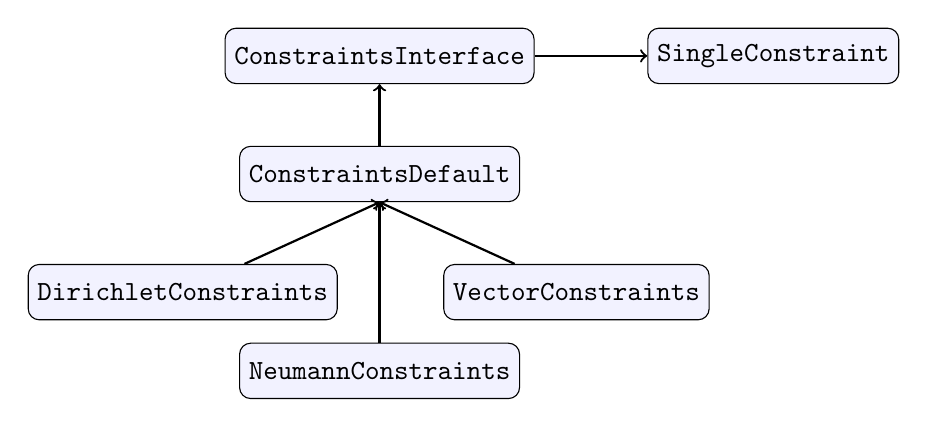
\begin{tikzpicture}
			\tikzstyle{boxs} = [draw, %text width=4em,
				fill=blue!5, minimum height=2em, rounded corners]
			\tikzstyle{boxsG} = [draw,  %text width=4em,
				fill=green!5, minimum height=2em, rounded corners ]
			\tikzstyle{line} = [draw,->,thick]
			\tikzstyle{lineR} = [draw,<-,thick]

			\tikzset{node distance = 50mm}
			\node(Functional)[boxs]{\CodeT{SingleConstraint}};

			\node(ConstraintsInterface)[boxs,left of = Functional]{\CodeT{ConstraintsInterface}} edge[line] (Functional.west);
			\tikzset{node distance = 15mm}
			\node(ConstraintsDefault)[boxs,below of = ConstraintsInterface]{\CodeT{ConstraintsDefault}} edge[line] (ConstraintsInterface.south);
			\tikzset{node distance = 30mm}
			\node(dummy1)[below of = ConstraintsInterface]{};
			\tikzset{node distance = 25mm}
			\node(DirichletConstraints)[boxs,left of = dummy1]{\CodeT{DirichletConstraints}} edge[line] (ConstraintsDefault.south);
			\node(NeumannConstraints)[boxs,below of = ConstraintsDefault]{\CodeT{NeumannConstraints}} edge[line] (ConstraintsDefault.south);
			\node(VectorConstraints)[boxs,right of = dummy1]{\CodeT{VectorConstraints}} edge[line] (ConstraintsDefault.south);

			\tikzset{node distance = 15mm}

		\end{tikzpicture}
	\end{remark}\theoremEndLine

	\begin{remark}[SingleConstraint vs. ConstraintsInterface]\theoremNewline
		The next figure shows the class concept again - concentrating on the difference between a single constraint and classes derived from the class \CodeT{ConstraintsInterface}. Here we should discuss about some implementation details, especially about the Interface class. (Is it convient to implement a method like \CodeT{applyLocal(en)}?)
% 		\begin{flushleft}
% 			\scalebox{0.6} % Change this value to rescale the drawing.
% 			{
% 			\begin{pspicture}(0,-10.9775)(23.0,10.550938)
% 			\rput{-90.0}(1.6625,15.4375){\psarc[linewidth=0.04](8.55,6.8875){3.85}{61.699245}{119.0546}}
% 			\rput{-270.0}(17.3375,-3.5625){\psarc[linewidth=0.04](10.45,6.8875){3.85}{61.699245}{119.0546}}
% 			\psframe[linewidth=0.04,dimen=outer](8.2,7.1375)(7.2,6.7375)
% 			\psframe[linewidth=0.04,dimen=outer,fillstyle=solid,fillcolor=red](9.4,7.1375)(8.4,6.7375)
% 			\psframe[linewidth=0.04,dimen=outer](10.6,7.1375)(9.6,6.7375)
% 			\psframe[linewidth=0.04,dimen=outer](11.8,7.1375)(10.8,6.7375)
% 			\psdots[dotsize=0.12](7.3,6.3375)
% 			\psdots[dotsize=0.12](7.7,6.3375)
% 			\psdots[dotsize=0.12](8.1,6.3375)
% 			\psdots[dotsize=0.12](8.5,6.3375)
% 			\psdots[dotsize=0.12](8.9,6.3375)
% 			\psdots[dotsize=0.12](9.3,6.3375)
% 			\psdots[dotsize=0.12](9.7,6.3375)
% 			\psdots[dotsize=0.12](10.1,6.3375)
% 			\psdots[dotsize=0.12](10.5,6.3375)
% 			\psdots[dotsize=0.12](11.0,6.3375)
% 			\psdots[dotsize=0.12](11.4,6.3375)
% 			\psdots[dotsize=0.12](11.8,6.3375)
% 			\psdots[dotsize=0.12](7.3,7.8375)
% 			\psdots[dotsize=0.12](7.7,7.8375)
% 			\psdots[dotsize=0.12](8.1,7.8375)
% 			\psdots[dotsize=0.12](8.5,7.8375)
% 			\psdots[dotsize=0.12](8.9,7.8375)
% 			\psdots[dotsize=0.12](9.3,7.8375)
% 			\psdots[dotsize=0.12](9.7,7.8375)
% 			\psdots[dotsize=0.12](10.1,7.8375)
% 			\psdots[dotsize=0.12](10.5,7.8375)
% 			\psdots[dotsize=0.12](11.0,7.8375)
% 			\psdots[dotsize=0.12](11.4,7.8375)
% 			\psdots[dotsize=0.12](11.8,7.8375)
% 			\usefont{T1}{ptm}{m}{n}
% 			\rput(7.992031,9.3475){\CodeT{SingleConstraint}}
% 			\usefont{T1}{ptm}{m}{n}
% 			\rput(8.932032,4.7475){\CodeT{applyLocal(en)}}
% 			\usefont{T1}{ptm}{m}{n}
% 			\rput(14.172031,6.9475){\CodeT{getRow()}}
% 			\psline[linewidth=0.04cm,arrowsize=0.05291667cm 2.0,arrowlength=1.4,arrowinset=0.4]{->}(13.2,7.0375)(12.5,7.0375)
% 			\psline[linewidth=0.04cm,arrowsize=0.05291667cm 2.0,arrowlength=1.4,arrowinset=0.4]{->}(15.3,7.0375)(16.3,7.0375)
% 			\psframe[linewidth=0.04,dimen=outer](8.0,0.5375)(7.0,0.1375)
% 			\psframe[linewidth=0.04,dimen=outer,fillstyle=solid,fillcolor=red](9.2,0.5375)(8.2,0.1375)
% 			\psframe[linewidth=0.04,dimen=outer](10.4,0.5375)(9.4,0.1375)
% 			\psframe[linewidth=0.04,dimen=outer](11.6,0.5375)(10.6,0.1375)
% 			\psframe[linewidth=0.04,dimen=outer](8.0,1.9375)(7.0,1.5375)
% 			\psframe[linewidth=0.04,dimen=outer,fillstyle=solid,fillcolor=red](9.2,1.9375)(8.2,1.5375)
% 			\psframe[linewidth=0.04,dimen=outer](10.4,1.9375)(9.4,1.5375)
% 			\psframe[linewidth=0.04,dimen=outer](11.6,1.9375)(10.6,1.5375)
% 			\psframe[linewidth=0.04,dimen=outer](8.0,-0.8625)(7.0,-1.2625)
% 			\psframe[linewidth=0.04,dimen=outer,fillstyle=solid,fillcolor=red](9.2,-0.8625)(8.2,-1.2625)
% 			\psframe[linewidth=0.04,dimen=outer](10.4,-0.8625)(9.4,-1.2625)
% 			\psframe[linewidth=0.04,dimen=outer](11.6,-0.8625)(10.6,-1.2625)
% 			\psdots[dotsize=0.12](7.1,-0.2625)
% 			\psdots[dotsize=0.12](7.5,-0.2625)
% 			\psdots[dotsize=0.12](7.9,-0.2625)
% 			\psdots[dotsize=0.12](8.3,-0.2625)
% 			\psdots[dotsize=0.12](8.7,-0.2625)
% 			\psdots[dotsize=0.12](9.1,-0.2625)
% 			\psdots[dotsize=0.12](9.5,-0.2625)
% 			\psdots[dotsize=0.12](9.9,-0.2625)
% 			\psdots[dotsize=0.12](10.3,-0.2625)
% 			\psdots[dotsize=0.12](10.8,-0.2625)
% 			\psdots[dotsize=0.12](11.2,-0.2625)
% 			\psdots[dotsize=0.12](11.6,-0.2625)
% 			\psdots[dotsize=0.12](7.1,0.9375)
% 			\psdots[dotsize=0.12](7.5,0.9375)
% 			\psdots[dotsize=0.12](7.9,0.9375)
% 			\psdots[dotsize=0.12](8.3,0.9375)
% 			\psdots[dotsize=0.12](8.7,0.9375)
% 			\psdots[dotsize=0.12](9.1,0.9375)
% 			\psdots[dotsize=0.12](9.5,0.9375)
% 			\psdots[dotsize=0.12](9.9,0.9375)
% 			\psdots[dotsize=0.12](10.3,0.9375)
% 			\psdots[dotsize=0.12](10.8,0.9375)
% 			\psdots[dotsize=0.12](11.2,0.9375)
% 			\psdots[dotsize=0.12](11.6,0.9375)
% 			\psline[linewidth=0.04cm,arrowsize=0.05291667cm 2.0,arrowlength=1.4,arrowinset=0.4]{->}(9.0,5.2375)(9.0,6.6375)
% 			\psdots[dotsize=0.12](7.3,8.1375)
% 			\psdots[dotsize=0.12](7.7,8.1375)
% 			\psdots[dotsize=0.12](8.1,8.1375)
% 			\psdots[dotsize=0.12](8.5,8.1375)
% 			\psdots[dotsize=0.12](8.9,8.1375)
% 			\psdots[dotsize=0.12](9.3,8.1375)
% 			\psdots[dotsize=0.12](9.7,8.1375)
% 			\psdots[dotsize=0.12](10.1,8.1375)
% 			\psdots[dotsize=0.12](10.5,8.1375)
% 			\psdots[dotsize=0.12](11.0,8.1375)
% 			\psdots[dotsize=0.12](11.4,8.1375)
% 			\psdots[dotsize=0.12](11.8,8.1375)
% 			\psdots[dotsize=0.12](7.3,8.4375)
% 			\psdots[dotsize=0.12](7.7,8.4375)
% 			\psdots[dotsize=0.12](8.1,8.4375)
% 			\psdots[dotsize=0.12](8.5,8.4375)
% 			\psdots[dotsize=0.12](8.9,8.4375)
% 			\psdots[dotsize=0.12](9.3,8.4375)
% 			\psdots[dotsize=0.12](9.7,8.4375)
% 			\psdots[dotsize=0.12](10.1,8.4375)
% 			\psdots[dotsize=0.12](10.5,8.4375)
% 			\psdots[dotsize=0.12](11.0,8.4375)
% 			\psdots[dotsize=0.12](11.4,8.4375)
% 			\psdots[dotsize=0.12](11.8,8.4375)
% 			\psdots[dotsize=0.12](7.3,6.0375)
% 			\psdots[dotsize=0.12](7.7,6.0375)
% 			\psdots[dotsize=0.12](8.1,6.0375)
% 			\psdots[dotsize=0.12](8.5,6.0375)
% 			\psdots[dotsize=0.12](8.9,6.0375)
% 			\psdots[dotsize=0.12](9.3,6.0375)
% 			\psdots[dotsize=0.12](9.7,6.0375)
% 			\psdots[dotsize=0.12](10.1,6.0375)
% 			\psdots[dotsize=0.12](10.5,6.0375)
% 			\psdots[dotsize=0.12](11.0,6.0375)
% 			\psdots[dotsize=0.12](11.4,6.0375)
% 			\psdots[dotsize=0.12](11.8,6.0375)
% 			\psdots[dotsize=0.12](7.3,5.7375)
% 			\psdots[dotsize=0.12](7.7,5.7375)
% 			\psdots[dotsize=0.12](8.1,5.7375)
% 			\psdots[dotsize=0.12](8.5,5.7375)
% 			\psdots[dotsize=0.12](8.9,5.7375)
% 			\psdots[dotsize=0.12](9.3,5.7375)
% 			\psdots[dotsize=0.12](9.7,5.7375)
% 			\psdots[dotsize=0.12](10.1,5.7375)
% 			\psdots[dotsize=0.12](10.5,5.7375)
% 			\psdots[dotsize=0.12](11.0,5.7375)
% 			\psdots[dotsize=0.12](11.4,5.7375)
% 			\psdots[dotsize=0.12](11.8,5.7375)
% 			\psdots[dotsize=0.12](7.3,5.4375)
% 			\psdots[dotsize=0.12](7.7,5.4375)
% 			\psdots[dotsize=0.12](8.1,5.4375)
% 			\psdots[dotsize=0.12](8.5,5.4375)
% 			\psdots[dotsize=0.12](8.9,5.4375)
% 			\psdots[dotsize=0.12](9.3,5.4375)
% 			\psdots[dotsize=0.12](9.7,5.4375)
% 			\psdots[dotsize=0.12](10.1,5.4375)
% 			\psdots[dotsize=0.12](10.5,5.4375)
% 			\psdots[dotsize=0.12](11.0,5.4375)
% 			\psdots[dotsize=0.12](11.4,5.4375)
% 			\psdots[dotsize=0.12](11.8,5.4375)
% 			\psdots[dotsize=0.12](7.3,7.5375)
% 			\psdots[dotsize=0.12](7.7,7.5375)
% 			\psdots[dotsize=0.12](8.1,7.5375)
% 			\psdots[dotsize=0.12](8.5,7.5375)
% 			\psdots[dotsize=0.12](8.9,7.5375)
% 			\psdots[dotsize=0.12](9.3,7.5375)
% 			\psdots[dotsize=0.12](9.7,7.5375)
% 			\psdots[dotsize=0.12](10.1,7.5375)
% 			\psdots[dotsize=0.12](10.5,7.5375)
% 			\psdots[dotsize=0.12](11.0,7.5375)
% 			\psdots[dotsize=0.12](11.4,7.5375)
% 			\psdots[dotsize=0.12](11.8,7.5375)
% 			\psdots[dotsize=0.12](7.1,1.2375)
% 			\psdots[dotsize=0.12](7.5,1.2375)
% 			\psdots[dotsize=0.12](7.9,1.2375)
% 			\psdots[dotsize=0.12](8.3,1.2375)
% 			\psdots[dotsize=0.12](8.7,1.2375)
% 			\psdots[dotsize=0.12](9.1,1.2375)
% 			\psdots[dotsize=0.12](9.5,1.2375)
% 			\psdots[dotsize=0.12](9.9,1.2375)
% 			\psdots[dotsize=0.12](10.3,1.2375)
% 			\psdots[dotsize=0.12](10.8,1.2375)
% 			\psdots[dotsize=0.12](11.2,1.2375)
% 			\psdots[dotsize=0.12](11.6,1.2375)
% 			\psdots[dotsize=0.12](7.1,-0.5625)
% 			\psdots[dotsize=0.12](7.5,-0.5625)
% 			\psdots[dotsize=0.12](7.9,-0.5625)
% 			\psdots[dotsize=0.12](8.3,-0.5625)
% 			\psdots[dotsize=0.12](8.7,-0.5625)
% 			\psdots[dotsize=0.12](9.1,-0.5625)
% 			\psdots[dotsize=0.12](9.5,-0.5625)
% 			\psdots[dotsize=0.12](9.9,-0.5625)
% 			\psdots[dotsize=0.12](10.3,-0.5625)
% 			\psdots[dotsize=0.12](10.8,-0.5625)
% 			\psdots[dotsize=0.12](11.2,-0.5625)
% 			\psdots[dotsize=0.12](11.6,-0.5625)
% 			\rput{-270.0}(10.3375,-9.9625){\psarc[linewidth=0.04](10.15,0.1875){3.85}{61.699245}{119.0546}}
% 			\rput{-90.0}(8.2625,8.6375){\psarc[linewidth=0.04](8.45,0.1875){3.85}{61.699245}{119.0546}}
% 			\usefont{T1}{ptm}{m}{n}
% 			\rput(9.032031,-1.9525){\CodeT{applyLocal(en)}}
% 			\psline[linewidth=0.04cm,fillcolor=red,arrowsize=0.05291667cm 2.0,arrowlength=1.4,arrowinset=0.4]{->}(8.4,-1.5625)(8.4,-1.2625)
% 			\psline[linewidth=0.04cm,fillcolor=red,arrowsize=0.05291667cm 2.0,arrowlength=1.4,arrowinset=0.4]{->}(8.6,-1.5625)(8.6,0.0375)
% 			\psline[linewidth=0.04cm,fillcolor=red,arrowsize=0.05291667cm 2.0,arrowlength=1.4,arrowinset=0.4]{->}(8.9,-1.5625)(8.9,1.4375)
% 			\usefont{T1}{ptm}{m}{n}
% 			\rput(8.282031,2.6475){\CodeT{DirichletConstraints}}
% 			\psframe[linewidth=0.04,dimen=outer,fillstyle=solid,fillcolor=red](18.3,0.7375)(17.3,0.3375)
% 			\psframe[linewidth=0.04,dimen=outer,fillstyle=solid,fillcolor=red](19.5,0.7375)(18.5,0.3375)
% 			\psframe[linewidth=0.04,dimen=outer,fillstyle=solid,fillcolor=red](20.7,0.7375)(19.7,0.3375)
% 			\psframe[linewidth=0.04,dimen=outer,fillstyle=solid,fillcolor=red](21.9,0.7375)(20.9,0.3375)
% 			\psframe[linewidth=0.04,dimen=outer,fillstyle=solid,fillcolor=red](18.3,2.1375)(17.3,1.7375)
% 			\psframe[linewidth=0.04,dimen=outer,fillstyle=solid,fillcolor=red](19.5,2.1375)(18.5,1.7375)
% 			\psframe[linewidth=0.04,dimen=outer,fillstyle=solid,fillcolor=red](20.7,2.1375)(19.7,1.7375)
% 			\psframe[linewidth=0.04,dimen=outer,fillstyle=solid,fillcolor=red](21.9,2.1375)(20.9,1.7375)
% 			\psframe[linewidth=0.04,dimen=outer,fillstyle=solid,fillcolor=red](18.3,-0.6625)(17.3,-1.0625)
% 			\psframe[linewidth=0.04,dimen=outer,fillstyle=solid,fillcolor=red](19.5,-0.6625)(18.5,-1.0625)
% 			\psframe[linewidth=0.04,dimen=outer,fillstyle=solid,fillcolor=red](20.7,-0.6625)(19.7,-1.0625)
% 			\psframe[linewidth=0.04,dimen=outer,fillstyle=solid,fillcolor=red](21.9,-0.6625)(20.9,-1.0625)
% 			\psdots[dotsize=0.12](17.4,-0.0625)
% 			\psdots[dotsize=0.12](17.8,-0.0625)
% 			\psdots[dotsize=0.12](18.2,-0.0625)
% 			\psdots[dotsize=0.12](18.6,-0.0625)
% 			\psdots[dotsize=0.12](19.0,-0.0625)
% 			\psdots[dotsize=0.12](19.4,-0.0625)
% 			\psdots[dotsize=0.12](19.8,-0.0625)
% 			\psdots[dotsize=0.12](20.2,-0.0625)
% 			\psdots[dotsize=0.12](20.6,-0.0625)
% 			\psdots[dotsize=0.12](21.1,-0.0625)
% 			\psdots[dotsize=0.12](21.5,-0.0625)
% 			\psdots[dotsize=0.12](21.9,-0.0625)
% 			\psdots[dotsize=0.12](17.4,1.1375)
% 			\psdots[dotsize=0.12](17.8,1.1375)
% 			\psdots[dotsize=0.12](18.2,1.1375)
% 			\psdots[dotsize=0.12](18.6,1.1375)
% 			\psdots[dotsize=0.12](19.0,1.1375)
% 			\psdots[dotsize=0.12](19.4,1.1375)
% 			\psdots[dotsize=0.12](19.8,1.1375)
% 			\psdots[dotsize=0.12](20.2,1.1375)
% 			\psdots[dotsize=0.12](20.6,1.1375)
% 			\psdots[dotsize=0.12](21.1,1.1375)
% 			\psdots[dotsize=0.12](21.5,1.1375)
% 			\psdots[dotsize=0.12](21.9,1.1375)
% 			\psdots[dotsize=0.12](17.4,1.4375)
% 			\psdots[dotsize=0.12](17.8,1.4375)
% 			\psdots[dotsize=0.12](18.2,1.4375)
% 			\psdots[dotsize=0.12](18.6,1.4375)
% 			\psdots[dotsize=0.12](19.0,1.4375)
% 			\psdots[dotsize=0.12](19.4,1.4375)
% 			\psdots[dotsize=0.12](19.8,1.4375)
% 			\psdots[dotsize=0.12](20.2,1.4375)
% 			\psdots[dotsize=0.12](20.6,1.4375)
% 			\psdots[dotsize=0.12](21.1,1.4375)
% 			\psdots[dotsize=0.12](21.5,1.4375)
% 			\psdots[dotsize=0.12](21.9,1.4375)
% 			\psdots[dotsize=0.12](17.4,-0.3625)
% 			\psdots[dotsize=0.12](17.8,-0.3625)
% 			\psdots[dotsize=0.12](18.2,-0.3625)
% 			\psdots[dotsize=0.12](18.6,-0.3625)
% 			\psdots[dotsize=0.12](19.0,-0.3625)
% 			\psdots[dotsize=0.12](19.4,-0.3625)
% 			\psdots[dotsize=0.12](19.8,-0.3625)
% 			\psdots[dotsize=0.12](20.2,-0.3625)
% 			\psdots[dotsize=0.12](20.6,-0.3625)
% 			\psdots[dotsize=0.12](21.1,-0.3625)
% 			\psdots[dotsize=0.12](21.5,-0.3625)
% 			\psdots[dotsize=0.12](21.9,-0.3625)
% 			\usefont{T1}{ptm}{m}{n}
% 			\rput(18.96203,-1.7525){\CodeT{apply()}}
% 			\rput{-270.0}(20.8375,-20.0625){\psarc[linewidth=0.04](20.45,0.3875){3.85}{61.699245}{119.0546}}
% 			\rput{-90.0}(18.3625,19.1375){\psarc[linewidth=0.04](18.75,0.3875){3.85}{61.699245}{119.0546}}
% 			\psframe[linewidth=0.04,dimen=outer,fillstyle=solid,fillcolor=red](18.0,7.2375)(17.0,6.8375)
% 			\psframe[linewidth=0.04,dimen=outer,fillstyle=solid,fillcolor=red](19.2,7.2375)(18.2,6.8375)
% 			\psframe[linewidth=0.04,dimen=outer,fillstyle=solid,fillcolor=red](20.4,7.2375)(19.4,6.8375)
% 			\psframe[linewidth=0.04,dimen=outer,fillstyle=solid,fillcolor=red](21.6,7.2375)(20.6,6.8375)
% 			\psdots[dotsize=0.12](17.1,6.4375)
% 			\psdots[dotsize=0.12](17.5,6.4375)
% 			\psdots[dotsize=0.12](17.9,6.4375)
% 			\psdots[dotsize=0.12](18.3,6.4375)
% 			\psdots[dotsize=0.12](18.7,6.4375)
% 			\psdots[dotsize=0.12](19.1,6.4375)
% 			\psdots[dotsize=0.12](19.5,6.4375)
% 			\psdots[dotsize=0.12](19.9,6.4375)
% 			\psdots[dotsize=0.12](20.3,6.4375)
% 			\psdots[dotsize=0.12](20.8,6.4375)
% 			\psdots[dotsize=0.12](21.2,6.4375)
% 			\psdots[dotsize=0.12](21.6,6.4375)
% 			\psdots[dotsize=0.12](17.1,7.9375)
% 			\psdots[dotsize=0.12](17.5,7.9375)
% 			\psdots[dotsize=0.12](17.9,7.9375)
% 			\psdots[dotsize=0.12](18.3,7.9375)
% 			\psdots[dotsize=0.12](18.7,7.9375)
% 			\psdots[dotsize=0.12](19.1,7.9375)
% 			\psdots[dotsize=0.12](19.5,7.9375)
% 			\psdots[dotsize=0.12](19.9,7.9375)
% 			\psdots[dotsize=0.12](20.3,7.9375)
% 			\psdots[dotsize=0.12](20.8,7.9375)
% 			\psdots[dotsize=0.12](21.2,7.9375)
% 			\psdots[dotsize=0.12](21.6,7.9375)
% 			\usefont{T1}{ptm}{m}{n}
% 			\rput(19.162031,4.8475){\CodeT{apply()}}
% 			\psline[linewidth=0.04cm,arrowsize=0.05291667cm 2.0,arrowlength=1.4,arrowinset=0.4]{->}(18.8,5.3375)(18.8,6.7375)
% 			\psdots[dotsize=0.12](17.1,8.2375)
% 			\psdots[dotsize=0.12](17.5,8.2375)
% 			\psdots[dotsize=0.12](17.9,8.2375)
% 			\psdots[dotsize=0.12](18.3,8.2375)
% 			\psdots[dotsize=0.12](18.7,8.2375)
% 			\psdots[dotsize=0.12](19.1,8.2375)
% 			\psdots[dotsize=0.12](19.5,8.2375)
% 			\psdots[dotsize=0.12](19.9,8.2375)
% 			\psdots[dotsize=0.12](20.3,8.2375)
% 			\psdots[dotsize=0.12](20.8,8.2375)
% 			\psdots[dotsize=0.12](21.2,8.2375)
% 			\psdots[dotsize=0.12](21.6,8.2375)
% 			\psdots[dotsize=0.12](17.1,8.5375)
% 			\psdots[dotsize=0.12](17.5,8.5375)
% 			\psdots[dotsize=0.12](17.9,8.5375)
% 			\psdots[dotsize=0.12](18.3,8.5375)
% 			\psdots[dotsize=0.12](18.7,8.5375)
% 			\psdots[dotsize=0.12](19.1,8.5375)
% 			\psdots[dotsize=0.12](19.5,8.5375)
% 			\psdots[dotsize=0.12](19.9,8.5375)
% 			\psdots[dotsize=0.12](20.3,8.5375)
% 			\psdots[dotsize=0.12](20.8,8.5375)
% 			\psdots[dotsize=0.12](21.2,8.5375)
% 			\psdots[dotsize=0.12](21.6,8.5375)
% 			\psdots[dotsize=0.12](17.1,6.1375)
% 			\psdots[dotsize=0.12](17.5,6.1375)
% 			\psdots[dotsize=0.12](17.9,6.1375)
% 			\psdots[dotsize=0.12](18.3,6.1375)
% 			\psdots[dotsize=0.12](18.7,6.1375)
% 			\psdots[dotsize=0.12](19.1,6.1375)
% 			\psdots[dotsize=0.12](19.5,6.1375)
% 			\psdots[dotsize=0.12](19.9,6.1375)
% 			\psdots[dotsize=0.12](20.3,6.1375)
% 			\psdots[dotsize=0.12](20.8,6.1375)
% 			\psdots[dotsize=0.12](21.2,6.1375)
% 			\psdots[dotsize=0.12](21.6,6.1375)
% 			\psdots[dotsize=0.12](17.1,5.8375)
% 			\psdots[dotsize=0.12](17.5,5.8375)
% 			\psdots[dotsize=0.12](17.9,5.8375)
% 			\psdots[dotsize=0.12](18.3,5.8375)
% 			\psdots[dotsize=0.12](18.7,5.8375)
% 			\psdots[dotsize=0.12](19.1,5.8375)
% 			\psdots[dotsize=0.12](19.5,5.8375)
% 			\psdots[dotsize=0.12](19.9,5.8375)
% 			\psdots[dotsize=0.12](20.3,5.8375)
% 			\psdots[dotsize=0.12](20.8,5.8375)
% 			\psdots[dotsize=0.12](21.2,5.8375)
% 			\psdots[dotsize=0.12](21.6,5.8375)
% 			\psdots[dotsize=0.12](17.1,5.5375)
% 			\psdots[dotsize=0.12](17.5,5.5375)
% 			\psdots[dotsize=0.12](17.9,5.5375)
% 			\psdots[dotsize=0.12](18.3,5.5375)
% 			\psdots[dotsize=0.12](18.7,5.5375)
% 			\psdots[dotsize=0.12](19.1,5.5375)
% 			\psdots[dotsize=0.12](19.5,5.5375)
% 			\psdots[dotsize=0.12](19.9,5.5375)
% 			\psdots[dotsize=0.12](20.3,5.5375)
% 			\psdots[dotsize=0.12](20.8,5.5375)
% 			\psdots[dotsize=0.12](21.2,5.5375)
% 			\psdots[dotsize=0.12](21.6,5.5375)
% 			\psdots[dotsize=0.12](17.1,7.6375)
% 			\psdots[dotsize=0.12](17.5,7.6375)
% 			\psdots[dotsize=0.12](17.9,7.6375)
% 			\psdots[dotsize=0.12](18.3,7.6375)
% 			\psdots[dotsize=0.12](18.7,7.6375)
% 			\psdots[dotsize=0.12](19.1,7.6375)
% 			\psdots[dotsize=0.12](19.5,7.6375)
% 			\psdots[dotsize=0.12](19.9,7.6375)
% 			\psdots[dotsize=0.12](20.3,7.6375)
% 			\psdots[dotsize=0.12](20.8,7.6375)
% 			\psdots[dotsize=0.12](21.2,7.6375)
% 			\psdots[dotsize=0.12](21.6,7.6375)
% 			\rput{-270.0}(27.3375,-13.1625){\psarc[linewidth=0.04](20.25,7.0875){3.85}{61.699245}{119.0546}}
% 			\rput{-90.0}(11.2625,25.4375){\psarc[linewidth=0.04](18.35,7.0875){3.85}{61.699245}{119.0546}}
% 			\psline[linewidth=0.04cm,fillcolor=red,arrowsize=0.05291667cm 2.0,arrowlength=1.4,arrowinset=0.4]{->}(18.4,5.3375)(17.6,6.7375)
% 			\psline[linewidth=0.04cm,fillcolor=red,arrowsize=0.05291667cm 2.0,arrowlength=1.4,arrowinset=0.4]{->}(19.3,5.3375)(19.8,6.7375)
% 			\psline[linewidth=0.04cm,fillcolor=red,arrowsize=0.05291667cm 2.0,arrowlength=1.4,arrowinset=0.4]{->}(19.5,5.3375)(20.9,6.7375)
% 			\psline[linewidth=0.04cm,fillcolor=red,arrowsize=0.05291667cm 2.0,arrowlength=1.4,arrowinset=0.4]{->}(18.0,-1.3625)(17.7,-1.1625)
% 			\psline[linewidth=0.04cm,fillcolor=red,arrowsize=0.05291667cm 2.0,arrowlength=1.4,arrowinset=0.4]{->}(18.1,-1.3625)(17.7,0.2375)
% 			\psline[linewidth=0.04cm,fillcolor=red,arrowsize=0.05291667cm 2.0,arrowlength=1.4,arrowinset=0.4]{->}(18.3,-1.3625)(17.9,1.6375)
% 			\psline[linewidth=0.04cm,fillcolor=red,arrowsize=0.05291667cm 2.0,arrowlength=1.4,arrowinset=0.4]{->}(18.6,-1.3625)(18.6,-1.1625)
% 			\psline[linewidth=0.04cm,fillcolor=red,arrowsize=0.05291667cm 2.0,arrowlength=1.4,arrowinset=0.4]{->}(18.8,-1.3625)(18.8,0.2375)
% 			\psline[linewidth=0.04cm,fillcolor=red,arrowsize=0.05291667cm 2.0,arrowlength=1.4,arrowinset=0.4]{->}(19.0,-1.3625)(19.0,1.6375)
% 			\psline[linewidth=0.04cm,fillcolor=red,arrowsize=0.05291667cm 2.0,arrowlength=1.4,arrowinset=0.4]{->}(19.2,-1.3625)(19.8,1.5375)
% 			\psline[linewidth=0.04cm,fillcolor=red,arrowsize=0.05291667cm 2.0,arrowlength=1.4,arrowinset=0.4]{->}(19.4,-1.3625)(20.1,0.2375)
% 			\psline[linewidth=0.04cm,fillcolor=red,arrowsize=0.05291667cm 2.0,arrowlength=1.4,arrowinset=0.4]{->}(19.6,-1.3625)(19.9,-1.1625)
% 			\psline[linewidth=0.04cm,fillcolor=red,arrowsize=0.05291667cm 2.0,arrowlength=1.4,arrowinset=0.4]{->}(19.9,-1.3625)(21.1,1.6375)
% 			\psline[linewidth=0.04cm,fillcolor=red,arrowsize=0.05291667cm 2.0,arrowlength=1.4,arrowinset=0.4]{->}(20.0,-1.3625)(21.1,0.2375)
% 			\psline[linewidth=0.04cm,fillcolor=red,arrowsize=0.05291667cm 2.0,arrowlength=1.4,arrowinset=0.4]{->}(20.1,-1.3625)(21.0,-1.1625)
% 			\psframe[linewidth=0.04,dimen=outer](23.0,10.0375)(5.5,-2.5625)
% 			\usefont{T1}{ptm}{m}{n}
% 			\rput(14.20875,10.3475){Systemmatrix}
% 			\usefont{T1}{ptm}{m}{n}
% 			\rput(14.156563,-3.5525){RHS}
% 			\usefont{T1}{ptm}{m}{n}
% 			\rput(8.292031,-4.5525){\CodeT{SingleConstraint}}
% 			\rput{-270.0}(2.8375,-16.2625){\psarc[linewidth=0.04](9.55,-6.7125){3.85}{61.699245}{119.0546}}
% 			\rput{-90.0}(10.5625,-2.8625){\psarc[linewidth=0.04](3.85,-6.7125){3.85}{61.699245}{119.0546}}
% 			\psframe[linewidth=0.04,dimen=outer](7.2,-5.0625)(6.2,-5.4625)
% 			\psframe[linewidth=0.04,dimen=outer](7.2,-8.0625)(6.2,-8.4625)
% 			\psframe[linewidth=0.04,dimen=outer,fillstyle=solid,fillcolor=red](7.2,-6.4625)(6.2,-6.8625)
% 			\psdots[dotsize=0.12](6.3,-5.7625)
% 			\psdots[dotsize=0.12](6.7,-5.7625)
% 			\psdots[dotsize=0.12](7.1,-5.7625)
% 			\psdots[dotsize=0.12](6.3,-6.0625)
% 			\psdots[dotsize=0.12](6.7,-6.0625)
% 			\psdots[dotsize=0.12](7.1,-6.0625)
% 			\psdots[dotsize=0.12](6.3,-7.1625)
% 			\psdots[dotsize=0.12](6.7,-7.1625)
% 			\psdots[dotsize=0.12](7.1,-7.1625)
% 			\psdots[dotsize=0.12](6.3,-7.6625)
% 			\psdots[dotsize=0.12](6.7,-7.6625)
% 			\psdots[dotsize=0.12](7.1,-7.6625)
% 			\usefont{T1}{ptm}{m}{n}
% 			\rput(9.472032,-6.6525){\CodeT{getRow()}}
% 			\psline[linewidth=0.04cm,arrowsize=0.05291667cm 2.0,arrowlength=1.4,arrowinset=0.4]{->}(8.5,-6.5625)(7.8,-6.5625)
% 			\psframe[linewidth=0.04,dimen=outer,fillstyle=solid,fillcolor=red](17.0,-4.9625)(16.0,-5.3625)
% 			\psframe[linewidth=0.04,dimen=outer,fillstyle=solid,fillcolor=red](17.0,-7.9625)(16.0,-8.3625)
% 			\psframe[linewidth=0.04,dimen=outer,fillstyle=solid,fillcolor=red](17.0,-6.3625)(16.0,-6.7625)
% 			\psdots[dotsize=0.12](16.1,-5.6625)
% 			\psdots[dotsize=0.12](16.5,-5.6625)
% 			\psdots[dotsize=0.12](16.9,-5.6625)
% 			\psdots[dotsize=0.12](16.1,-5.9625)
% 			\psdots[dotsize=0.12](16.5,-5.9625)
% 			\psdots[dotsize=0.12](16.9,-5.9625)
% 			\psdots[dotsize=0.12](16.1,-7.0625)
% 			\psdots[dotsize=0.12](16.5,-7.0625)
% 			\psdots[dotsize=0.12](16.9,-7.0625)
% 			\psdots[dotsize=0.12](16.1,-7.5625)
% 			\psdots[dotsize=0.12](16.5,-7.5625)
% 			\psdots[dotsize=0.12](16.9,-7.5625)
% 			\rput{-90.0}(20.2625,7.0375){\psarc[linewidth=0.04](13.65,-6.6125){3.85}{61.699245}{119.0546}}
% 			\rput{-270.0}(12.7375,-25.9625){\psarc[linewidth=0.04](19.35,-6.6125){3.85}{61.699245}{119.0546}}
% 			\usefont{T1}{ptm}{m}{n}
% 			\rput(16.582031,-4.4525){\CodeT{DirichletConstraints}}
% 			\psframe[linewidth=0.04,dimen=outer](23.0,-3.9625)(5.5,-9.4625)
% 			\usefont{T1}{ptm}{m}{n}
% 			\rput(6.8620315,-8.8525){\CodeT{apply()}}
% 			\usefont{T1}{ptm}{m}{n}
% 			\rput(16.46203,-8.8525){\CodeT{apply()}}
% 			\psline[linewidth=0.04cm,fillcolor=red,arrowsize=0.05291667cm 2.0,arrowlength=1.4,arrowinset=0.4]{->}(6.5,-8.6625)(6.5,-6.9625)
% 			\psline[linewidth=0.04cm,fillcolor=red,arrowsize=0.05291667cm 2.0,arrowlength=1.4,arrowinset=0.4]{->}(16.1,-8.5625)(16.1,-8.3625)
% 			\psline[linewidth=0.04cm,fillcolor=red,arrowsize=0.05291667cm 2.0,arrowlength=1.4,arrowinset=0.4]{->}(16.3,-8.5625)(16.3,-6.8625)
% 			\psline[linewidth=0.04cm,fillcolor=red,arrowsize=0.05291667cm 2.0,arrowlength=1.4,arrowinset=0.4]{->}(16.6,-8.5625)(16.6,-5.4625)
% 			\psframe[linewidth=0.04,dimen=outer](9.3,-9.8625)(8.3,-10.2625)
% 			\usefont{T1}{ptm}{m}{n}
% 			\rput(12.065937,-10.0525){= entity with boundary faces}
% 			\psdots[dotsize=0.12](8.8,-10.7625)
% 			\usefont{T1}{ptm}{m}{n}
% 			\rput(12.355938,-10.7525){= entity without boundary faces}
% 			\end{pspicture}
% 			}
% 		\end{flushleft}
	\end{remark}\theoremEndLine


	\begin{class}[\CodeT{SingleConstraint< FunctionalImp >}]
		Represents a single constraint. Mainly, this class is the formal implementation of \ref{definition::abstract_concept::constraint}. This class is the basic class for all other classes dealing with constraints. Normally this class is not used directly because an efficient implementation is not possible.\\
		Shortly said, a single constraint presents a pair of a \emph{functional} (defining the constraint) and \emph{row number} determing the row which has to be deleted in the system matrix.\\
		This means, that a class (for example representing the dirichlet constraints) can be (formally) seen as a vector of \CodeT{SingleConstraints}.
		\\\\
      \begin{tabular}{|l|l|}
        \hline
        \CodeT{number} & Computes $F[v]$, where $F$ is the functional and $v$\\
        \CodeT{ = operator( discretefunction )} & the discrete function.\\
        \hline
				\CodeT{vector} & just calls \CodeT{applyLocal()} for each entity.\\
				\CodeT{ = apply( discreteFunction) } & \\
				\hline
        \CodeT{localVector} & \\
        \CodeT{ = applyLocal( entity,} & \\
        \CodeT{ localBasefunctionSet )}  & \\
        \hline
				\CodeT{int} & returns the row number which has to be deleted \\
				\CodeT{ = getRow()} & in the system matrix.\\
        \hline
				\CodeT{functional} & returns the functional representing the constraint,\\
				\CodeT{ = getFunctional()} & i.e. $F[v]\stackrel{!}{=}0$ for the functional $F$\\
				  & returned by this function.\\
				\hline
      \end{tabular}
    \end{class}\theoremEndLine

	\begin{class}[\CodeT{ConstraintsInterface< FunctionalImp >}]
		This class represents an interface for all classes. Mention that it is possible to write something like this: \CodeT{ConstraintsInterfaceImp C; C[i].apply();}.
		\\\\
      \begin{tabular}{|l|l|}
        \hline
        \CodeT{number} & Computes $F[v]$, where $F$ is the functional and $v$\\
        \CodeT{ = operator( discretefunction )} & the discrete function.\\
        \hline
				\CodeT{vector} & just calls \CodeT{applyLocal()} for each entity.\\
				\CodeT{ = apply( discreteFunction) } & \\
				\hline
        \CodeT{localVector} & \\
        \CodeT{ = applyLocal( entity,} & \\
        \CodeT{ localBasefunctionSet )}  & \\
        \hline
				\CodeT{int} & Returns number of constraints. \\
				\CodeT{ = size()} & \\
				\hline
				\CodeT{singleconstraint} & Returns a single constraint represented\\
				\CodeT{ = operator[i]} & by the class \CodeT{SingleConstraint}. This \\
					& method will not be used in general.\\
				\hline
      \end{tabular}
    \end{class}\theoremEndLine

	\begin{class}[\CodeT{ConstraintsDefault< FunctionalImp >}]
		Default implementation of \CodeT{ConstraintsInterface}.
  \end{class}\theoremEndLine

	\begin{class}[\CodeT{DirichletConstraints< FunctionalImp >}]
		An example for constraints: Implementation of Dirichlet constraints.\\
		Derived from \CodeT{ConstraintsDefault}. Here we will \emph{overwrite} the methods \CodeT{operator()}, \CodeT{apply()} and \CodeT{applyLocal()} without using the single constraints from \CodeT{SingleConstraint}.\\\\
		\begin{tabular}{|l|l|}
			\hline
			\CodeT{number} & Computes $F[v]$, where $F$ is the functional and $v$\\
			\CodeT{ = operator( discretefunction )} & the discrete function.\\
			\hline
			\CodeT{vector} & just calls \CodeT{applyLocal()} for each entity.\\
			\CodeT{ = apply( discreteFunction) } & \\
			\hline
			\CodeT{localVector} & \\
			\CodeT{ = applyLocal( entity,} & \\
			\CodeT{ localBasefunctionSet )}  & \\
			\hline
			\CodeT{int} & Returns number of constraints. \\
			\CodeT{ = size()} & \\
			\hline
			\CodeT{singleconstraint} & Returns a single constraint represented\\
			\CodeT{ = operator[i]} & by the class \CodeT{SingleConstraint}. This \\
				& method will not be used in general.\\
			\hline
		\end{tabular}
  \end{class}\theoremEndLine

	\begin{class}[\CodeT{NeumannConstraints< FunctionalImp >}]
		An example for constraints: Implementation of Neumann constraints.\\
		Derived from \CodeT{ConstraintsDefault}. See above.
  \end{class}\theoremEndLine

	\begin{class}[\CodeT{VectorConstraints< FunctionalImp >}]
		An example for constraints: Here the constraints are stored explicitly in a vector of elements from the class \CodeT{SingleConstraint}. Derived from \CodeT{ConstraintsDefault}. \emph{In general we do not want to have such a class}.
  \end{class}\theoremEndLine


%(Operator ( Subspace, ProblemInfo ))(u) = Functional


  \bibliographystyle{plain}
  \bibliography{dune-fem-functionals}


\end{document}




